\documentclass[12pt,aspectratio=1610]{beamer}
\RequirePackage{
    amsmath,
    amssymb,
    calc,
    cancel,
    booktabs,
    color,
    siunitx,
    tikz,
    wrapfig,
    array,
    leftidx,
    float,
    etoolbox,
    fancyhdr,
    longtable,
    hyperref,
    ltcaption,
    ulem,
    wasysym,
    accents,
}

\sisetup{
    detect-all              = true,
    separate-uncertainty    = true,                                   % 7.2 ± 0.5
    multi-part-units        = single,
    per-mode                = reciprocal,                   % symbol for "m/s", reciprocal for "ms^{-1}"
    group-separator         = {\,},
    group-minimum-digits    = 5,
    inter-unit-product      = {\kern 0.10em},
    exponent-product        = \cdot,                        % \times for 5 × 10^7, \cdot for 5 . 1O^7    
    number-unit-product     = {\ },
    output-decimal-marker   = {\text{.}},
    range-units             = single,
    range-phrase            = {\text{ -- }},
    list-units              = single,
    list-final-separator    = {\text{\ a\ }},
    retain-explicit-plus    = true,
}

\hypersetup{
    hidelinks,
    breaklinks              = true,
}

\usepackage[
    final
]{pdfpages}

\usepackage[many]{tcolorbox}
\RenewDocumentCommand{\vec}{m}{\overrightarrow{#1}}

\makeatletter
    \def\new@mathgroup{\alloc@8\mathgroup\mathchardef\@cclvi}
    \patchcmd{\document@select@group}{\sixt@@n}{\@cclvi}{}{}
    \patchcmd{\select@group}{\sixt@@n}{\@cclvi}{}{}
\makeatother

\RequirePackage{mathspec}                                   % includes fontspec
\RequirePackage{polyglossia}                                % multi-language support
\RequirePackage{xunicode}
\setdefaultlanguage{slovak}

% Setup fonts -- see fontspec/mathspec documentation.
% Fonts are loaded from .ttf and .otf files in the core/fonts/ directory. We NEVER use system fonts.
\defaultfontfeatures{
    Mapping         = tex-text,
    Scale           = MatchLowercase,
    Ligatures       = TeX
}

\DeclareSIUnit\au{AU}
\DeclareSIUnit\pixel{px}
\DeclareSIUnit\lightyear{ly}
\DeclareSIUnit\parsec{pc}
\DeclareSIUnit\earthmass{M_{\earth}}
\DeclareSIUnit\speedoflight{c}
\DeclareSIUnit\foe{foe}
\DeclareSIUnit\year{yr}
\DeclareSIUnit\eur{€}
\DeclareSIUnit\solarmass{M_{\astrosun}}
\DeclareSIUnit\solarluminosity{L_{\astrosun}}
\DeclareSIUnit{\byte}{B}

\DeclareMathOperator{\diff}{\mathrm{d}\!}
\DeclareMathOperator{\pdiff}{\partial\!}

\NewDocumentCommand{\slashfrac}{m m}{\left.#1\middle/#2\right.}
\NewDocumentCommand{\derive}{O{} m m}{\frac{\mathop{\mathrm{d}^{#1}#2}}{\mathop{\mathrm{d}#3^{#1}}}}
%\NewDocumentCommand{\derive}{O{} m m}{\frac{\diffe^{#1}#2}{\diffe#3^{#1}}}
\NewDocumentCommand{\pderive}{O{} m m}{\frac{\partial^{#1} #2}{\partial #3^{#1}}}

\NewDocumentCommand{\integrate}{O{} O{} m m}{\int\limits_{#1}^{#2} \! #3 \, \diff#4}
\NewDocumentCommand{\iintegrate}{O{} O{} m m m}{\iint\limits_{#1}^{\quad#2} #3 \d#4\!\d#5}
\NewDocumentCommand{\iiintegrate}{O{} O{} m m m m}{\iiint\limits_{#1}^{\quad#2} #3 \d#4\!\d#5\!\d#6}

\NewDocumentCommand{\labelmath}{m +m}{%
    \begin{equation}%
        #2%
        \label{#1}%
    \end{equation}%
}

\NewDocumentCommand{\labelalign}{m +m}{%
    \begin{align}%
        #2%
        \label{#1}%
    \end{align}%
}

\linespread{1.0}
\setlength{\parindent}{0cm}
\setlength{\parskip}{6pt}
\setlength{\abovedisplayskip}{0mm}
\setlength{\belowdisplayskip}{0mm}
\setlength{\abovedisplayshortskip}{0mm}
\setlength{\belowdisplayshortskip}{0mm}
\setlength{\itemindent}{0pt}
\setlength{\textfloatsep}{0mm}
\setlength{\tabcolsep}{3mm}
\setlength{\LTcapwidth}{0.8\textwidth}
\renewcommand{\arraystretch}{1.2}

\setcounter{secnumdepth}{2}
\linespread{1.0}
\setlength{\parindent}{0cm}
\setlength{\parskip}{6pt}
\setlength{\abovedisplayskip}{0mm}
\setlength{\belowdisplayskip}{0mm}
\setlength{\abovedisplayshortskip}{0mm}
\setlength{\belowdisplayshortskip}{0mm}
\setlength{\itemindent}{0pt}
\setlength{\textfloatsep}{0mm}
\setlength{\tabcolsep}{3mm}
\renewcommand{\arraystretch}{1.2}

\setcounter{secnumdepth}{0}

\NewDocumentCommand{\fspicture}{m O{W} O{black}}{
    {
        \setbeamertemplate{navigation symbols}{}
        \setbeamercolor{background canvas}{bg = #3}
        \begin{frame}[plain]
            \begin{tikzpicture}[remember picture, overlay]
                \node[at=(current page.center)] {
                    \ifstrequal{H}{#2}{                                  
                        \includegraphics[height=\paperheight]{#1}%
                    }{%
                        \includegraphics[width=\paperwidth]{#1}%
                    }
                };
            \end{tikzpicture}
        \end{frame}
    }
}

\NewDocumentCommand{\frejm}{m +m}{
    \begin{frame}
        \frametitle{#1}
        #2
    \end{frame}
}
\defbeamertemplate{description item}{align center}{\hfill\insertdescriptionitem\hfill}
\definecolor{desc}{rgb}{0.66, 0, 0}
\definecolor{citem}{rgb}{0.72, 0, 0}
\definecolor{csitem}{rgb}{0.90, 0, 0}
\definecolor{cssitem}{rgb}{1, 0.1, 0.1}
\definecolor{qprimarybg}{rgb}{0.95, 0.95, 0.95}
\definecolor{check}{rgb}{0, 0.8, 0}

\setbeamertemplate{navigation symbols}{}
\newfontfamily{\semibold}{Segoe UI Semibold}
\RenewDocumentCommand{\emph}{m}{{\semibold#1}}

\mode<presentation> {
    \usetheme{Szeged}
    \usecolortheme{beaver}
    
    \usefonttheme{professionalfonts}
    \setallmainfonts{Minion Pro}
    \setmathrm{Minion Pro}
    
    \setsansfont{Segoe UI}
    \setmonofont{Consolas}
    \setbeamercolor*{enumerate item}{fg = citem}
    \setbeamercolor*{enumerate subitem}{fg = csitem}
    \setbeamercolor*{enumerate subsubitem}{fg = cssitem}
    \setbeamercolor*{description item}{fg = desc}
    \setbeamercolor*{itemize item}{fg = citem}
    \setbeamercolor*{itemize subitem}{fg = csitem}
    \setbeamercolor*{itemize subsubitem}{fg = cssitem}
    \setbeamercolor*{palette primary}{fg = red, bg = qprimarybg}
}

\AtBeginSection[]{
    \subsection{\insertsection}
    \begin{frame}
        \vfill
        \centering
        \begin{beamercolorbox}[sep = 8pt, center, shadow = true, rounded = true]{title}
            \usebeamerfont{title}\insertsectionhead\\[1.5mm]%
            \vfill
        \end{beamercolorbox}
        \vfill
    \end{frame}
}
\makeatletter

% Render percent sign with nice font, not ugly Computer modern
    \mathcode`\%="7025

% Fixes mathspec bug -- URL numbers are rendered with wrong font
    \ernewcommand\eu@MathPunctuation@symfont{Latin:m:n}
    \DeclareMathSymbol{,}{\mathpunct}{\eu@MathPunctuation@symfont}{`,}
    \DeclareMathSymbol{.}{\mathord}{\eu@MathPunctuation@symfont}{`.}
    \DeclareMathSymbol{<}{\mathrel}{\eu@MathPunctuation@symfont}{`<}
    \DeclareMathSymbol{>}{\mathrel}{\eu@MathPunctuation@symfont}{`>}
    \DeclareMathSymbol{/}{\mathord}{\eu@MathPunctuation@symfont}{`/}
    \DeclareMathSymbol{;}{\mathpunct}{\eu@MathPunctuation@symfont}{`;}
    \DeclareMathSymbol{(}{\mathopen}{\eu@DigitsArabic@symfont}{`(}
    \DeclareMathSymbol{)}{\mathclose}{\eu@DigitsArabic@symfont}{`)}
    \XeTeXDeclareMathSymbol{^^^^2026}{\mathinner}{\eu@MathPunctuation@symfont}{"2026}[\mathellipsis]
    \DeclareMathSymbol{0}{\mathalpha}{\eu@DigitsArabic@symfont}{`0}
    \DeclareMathSymbol{1}{\mathalpha}{\eu@DigitsArabic@symfont}{`1}
    \DeclareMathSymbol{2}{\mathalpha}{\eu@DigitsArabic@symfont}{`2}
    \DeclareMathSymbol{3}{\mathalpha}{\eu@DigitsArabic@symfont}{`3}
    \DeclareMathSymbol{4}{\mathalpha}{\eu@DigitsArabic@symfont}{`4}
    \DeclareMathSymbol{5}{\mathalpha}{\eu@DigitsArabic@symfont}{`5}
    \DeclareMathSymbol{6}{\mathalpha}{\eu@DigitsArabic@symfont}{`6}
    \DeclareMathSymbol{7}{\mathalpha}{\eu@DigitsArabic@symfont}{`7}
    \DeclareMathSymbol{8}{\mathalpha}{\eu@DigitsArabic@symfont}{`8}
    \DeclareMathSymbol{9}{\mathalpha}{\eu@DigitsArabic@symfont}{`9}
\makeatother


\usepackage{tabularx}

\AtBeginSection[]{
    \begin{frame}
        \vfill
        \centering
        \begin{beamercolorbox}[sep = 8pt, center, shadow = true, rounded = true]{title}
            \usebeamerfont{title}\insertsectionhead\\[5mm]%
            \vfill
        \end{beamercolorbox}
        \vfill
    \end{frame}
}

\makeatletter
\mode<presentation> {
    \usetheme{Szeged}
    \usecolortheme{beaver}
    
    \usefonttheme{professionalfonts}
    \setallmainfonts{Minion Pro}
    \setmathrm{Minion Pro}
    
    \setsansfont{Segoe UI}
    \setmonofont{Consolas}
    \setbeamercolor*{enumerate item}{fg = citem}
    \setbeamercolor*{enumerate subitem}{fg = csitem}
    \setbeamercolor*{enumerate subsubitem}{fg = cssitem}
    \setbeamercolor*{description item}{fg = desc}
    \setbeamercolor*{itemize item}{fg = citem}
    \setbeamercolor*{itemize subitem}{fg = csitem}
    \setbeamercolor*{itemize subsubitem}{fg = cssitem}
    \setbeamercolor*{palette primary}{fg = red, bg = qprimarybg}
}

\title{Determination of Meteoroid Flux from Meteor Data after Debiasing by Numerical Simulation}
\author{\small \emph{Martin Baláž} \\ Juraj Tóth, PhD. \\ Peter Vereš, PhD. \\ Robert Jedicke, PhD.}
\institute{Meteoroids 2019, Bratislava}
\date{2019--06--18}

\begin{document}
    {
        \usebackgroundtemplate{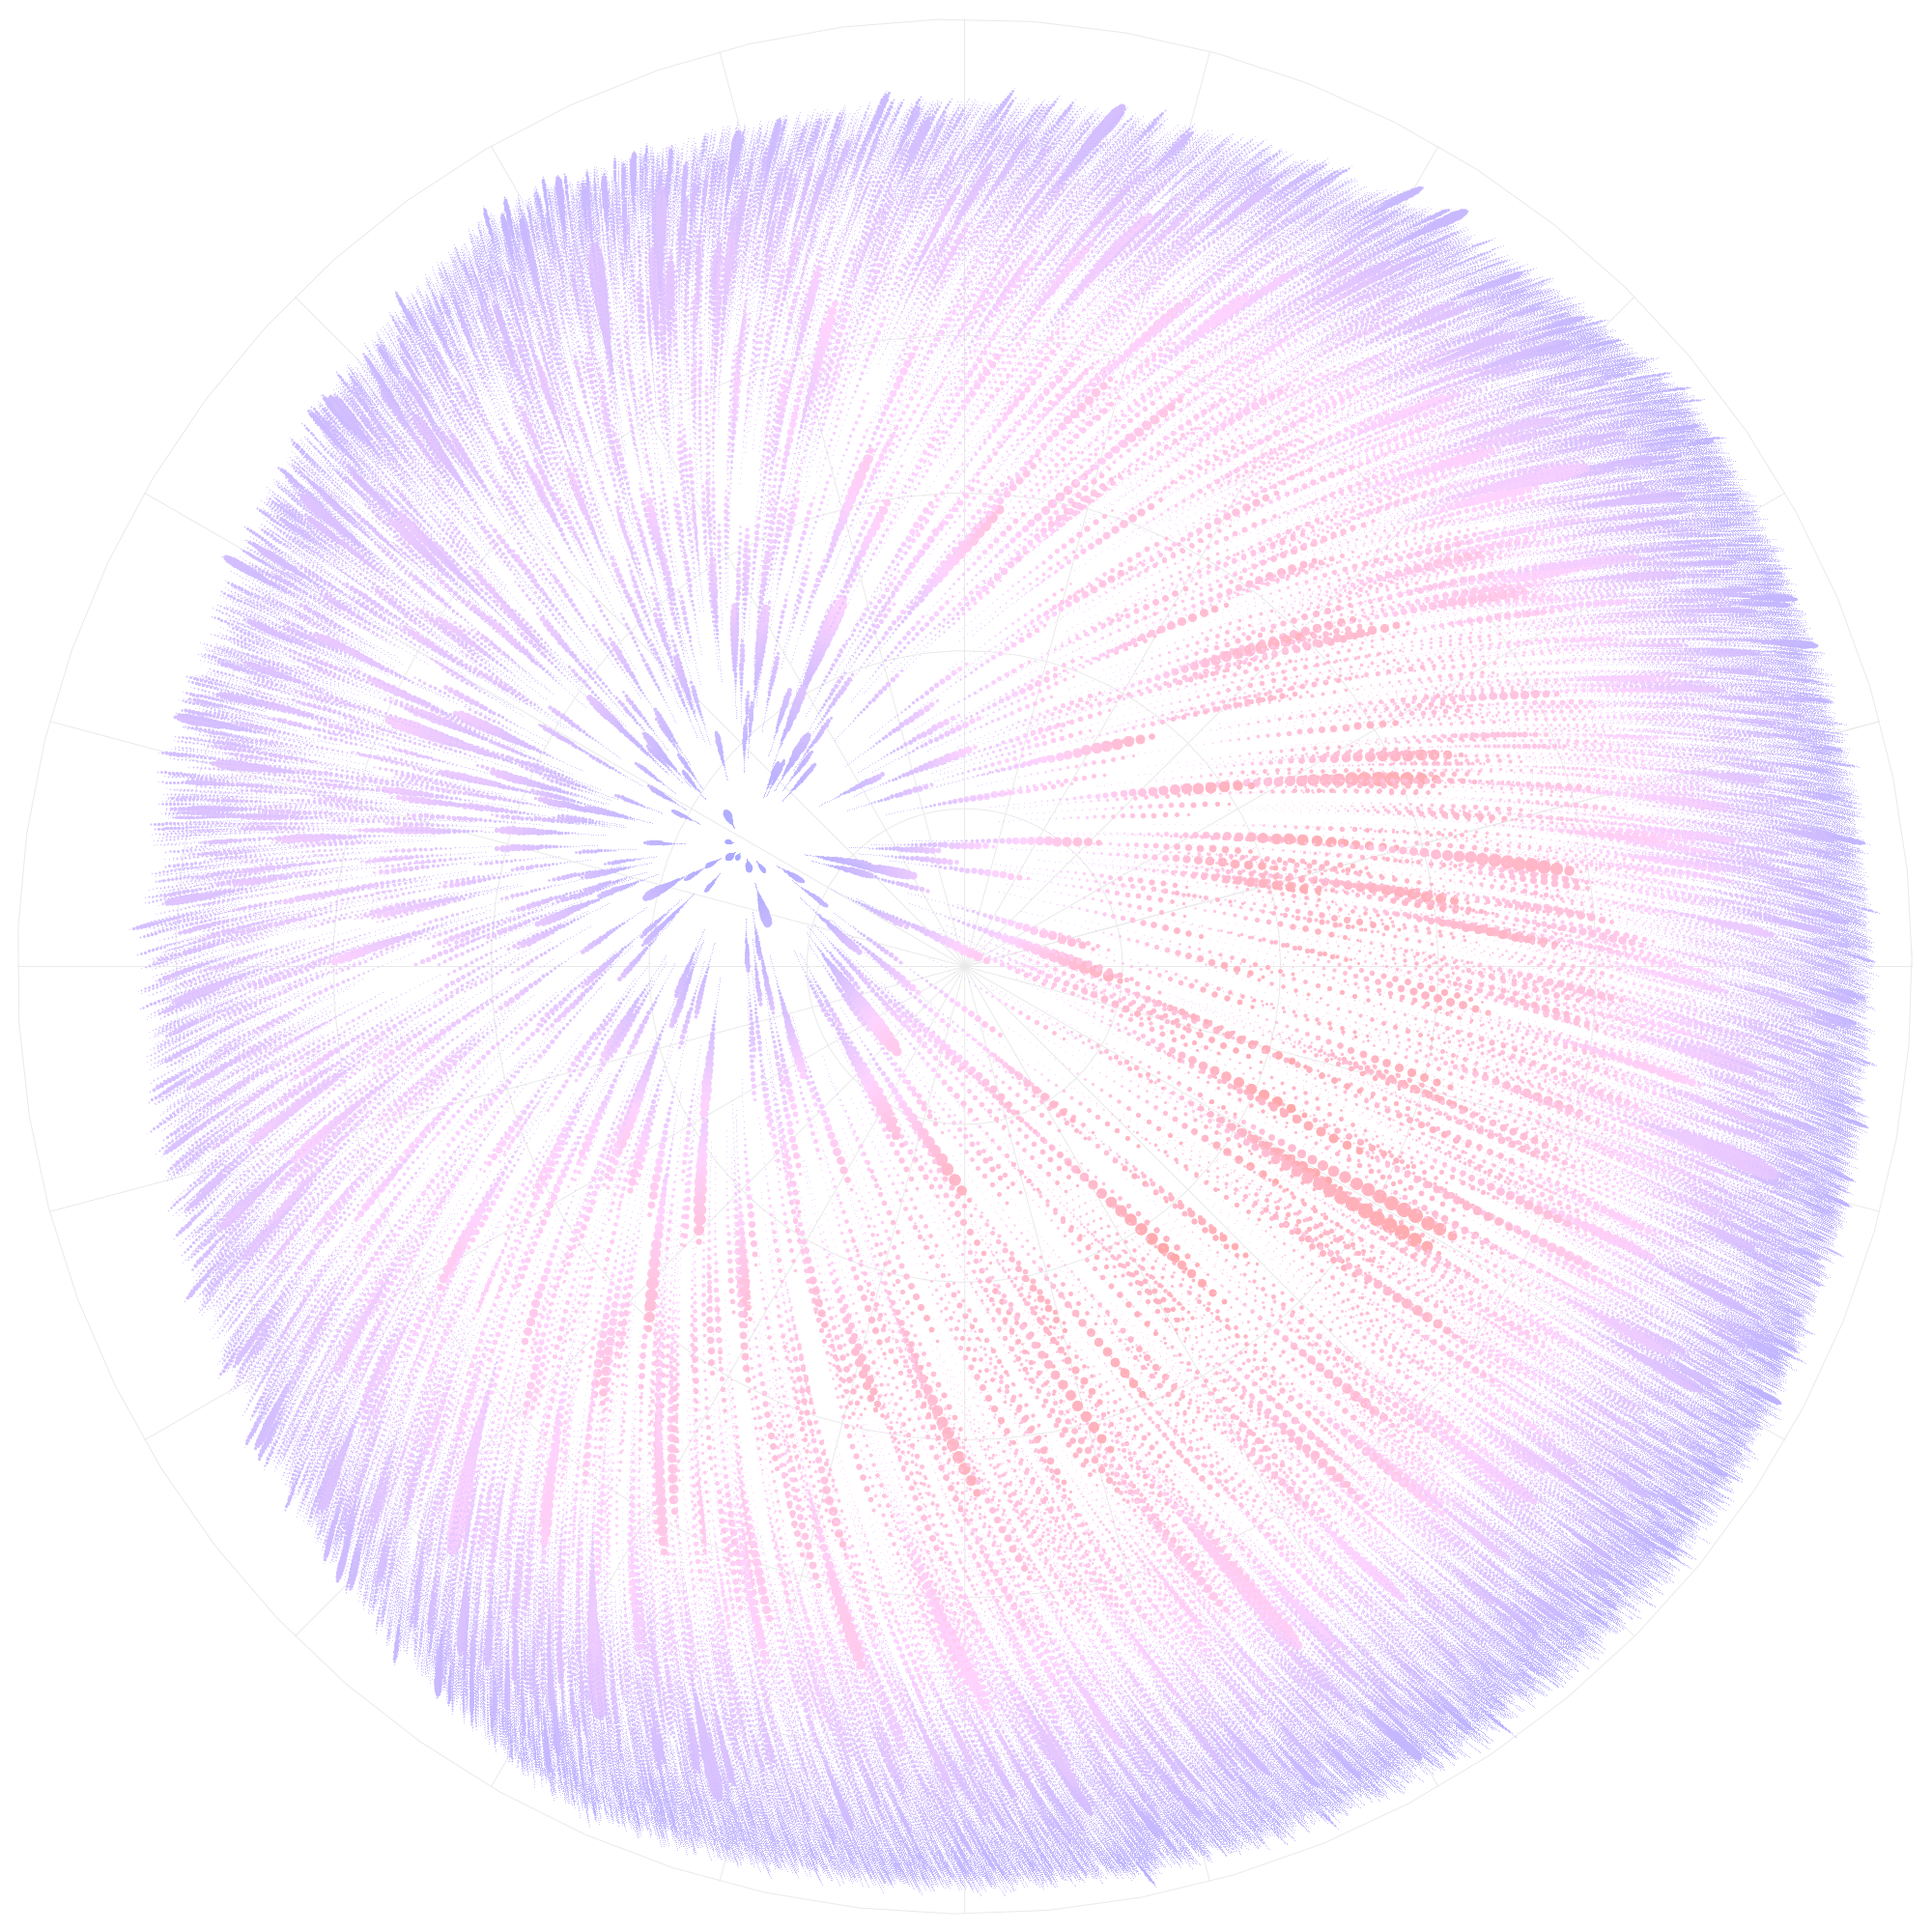
\includegraphics[width=\paperwidth]{fireworks-i.png}}
        \begin{frame}
            \titlepage
        \end{frame}
    }
                
    \section{Overview}
		\subsection{Overview}
			\frejm{Objective}{
                To \emph{determine} the total meteoroid flux utilizing data from \emph{AMOS}\\[4mm]
				\pause
                \emph{Problem}: data is severely distorted by selection bias\\[4mm]
                \pause
                \emph{Solution}: \emph{extrapolate} from collected data
                    \begin{itemize}
                        \item analyze the detection ability of AMOS
                        \item calibrate the system
                        \item \emph{de-bias} the observations
                    \end{itemize}
				\vspace{5mm}
				\pause
				Let us \emph{simulate} the population and try to match it to the data!
			}
			
			\frejm{Algorithm}{
				\begin{enumerate}
					\item generate the meteoroid population
					\pause
					\item simulate atmospheric entry and create meteor objects
					\pause
					\item compute meteor sightings as seen by predefined observers
						\begin{itemize}
							\item position in the sky, magnitude, entry angle, ...
						\end{itemize}
					\pause
					\item apply observational bias 
						\begin{itemize}
							\item limiting magnitude, altitude, angular speed, ...
						\end{itemize}
                    \pause
					\item calculate the statistic and compare it to AMOS data 
					\item adjust bias parameters 
					\pause
					\item repeat
				\end{enumerate}
			}
						
    \setbeamersize{description width = 5mm}
    \section{Simulation}
        \subsection{Simulation}
            \frejm{Model}{            
                \emph{Whipple} (1938), improved by \emph{Öpik} (1955) and \emph{Ceplecha} (2001)
                
                We assume
                \begin{itemize}
                    \item spherical, continuously ablating particles
                    \item no gravity
                \end{itemize}
                
                We need
                \begin{itemize}
                    \item equations of motion
                    \item equation of luminance
                    \item atmospheric and instrumental effects
                    \item to compute the statistic
                \end{itemize}            
            }
        
            %\frejm{Equations of motion}{
            %    \begin{itemize}
            %        \item braking equation
            %        $$
            %            \diff{v} = -\frac{\Gamma A}{m^{1/3} \rho^{2/3}} \rho_{\mathrm{air}} v^2 \diff{t}
            %        $$
            %        \item equation of ablation
            %        $$
            %            \diff{m} = -\frac{\Lambda A}{2Q} \frac{m^{2/3}}{\rho^{2/3}} \rho_{\mathrm{air}} v^3 \diff{t}
            %        $$
            %        \item equation of luminance
            %        $$
            %            L = \tau(v) \frac{\Lambda A}{4Q} \frac{m^{2/3}}{\rho^{2/3}} \rho_{\mathrm{air}} v^5
            %        $$
            %        \begin{itemize}
            %            \item $\tau(v)$ determined by \emph{Jones \& Halliday (2001)}
            %        \end{itemize}
            %    \end{itemize}
            %}
            
            \frejm{Simulation of flight}{
                Customized \emph{Runge--Kutta} integrator (RK4)
                \begin{itemize}
                    \item run until complete ablation of the particle
                    \item \emph{snapshots} taken 20 times per second
                    \item multiple integration steps between snapshots
                \end{itemize}
            }
            
            \frejm{Virtual observations}{
                Next, we create observations
                \begin{itemize}
                    \item observers on the ground
                    \begin{itemize}
                        \item each represents an AMOS camera
                    \end{itemize}
                    \item sequence of frames
                \end{itemize}           
            }
                
            \fspicture{angularSpeed-teplicne-streaks.png}[H][black]
            
            \frejm{Virtual observations}{
                Next, we create observations
                \begin{itemize}
                    \item observers on the ground
                    \begin{itemize}
                        \item each represents an AMOS camera
                    \end{itemize}
                    \item sequence of frames
                    \item only the \emph{brightest frame} is analyzed
                \end{itemize}           
            }
            \fspicture{angularSpeed-teplicne-streaks.png}[H][black]
            \fspicture{angularSpeed-teplicne-dots.png}[H][black]
                
            \frejm{Selection bias}{
                \emph{Detection efficiency is not constant!}            
                \begin{itemize}
                    \item probability of detection is higher for meteors that are
                    \begin{itemize}
                        \item brighter
                        \item slower
                        \item closer to zenith
                        \item ...
                    \end{itemize}
                    \pause
                    \item for each meteor \emph{decide} whether it is \emph{detected}
                    \item compare visible meteors to real data
                \end{itemize}
            }
            
            \fspicture{angularSpeed-teplicne-dots.png}[H][black]
            \fspicture{angularSpeed-teplicne-biased.png}[H][black]

            \fspicture{limmag.pdf}[H][white]
                            
			\frejm{Tool: ASMODEUS}{
                \textbf{A}ll-\textbf{S}ky \textbf{M}eteor \textbf{O}ptical \textbf{D}etection \textbf{E}fficiency \textbf{S}imulator\\[5mm]
                A multi-purpose virtual meteor observatory
				\begin{itemize}
					\item suite of seven scripts in \emph{Python}
					\item implements the described model
                    \item numerous analysis and visualisation tools
				\end{itemize}
			}
            
            %\fspicture{mjd-entryAngle-appMag.png}
            %\fspicture{logInitMass-absMag-appMag.png}
            %\fspicture{absMag-elevation-appMag.png}

    \section{Flux}
        \subsection{Flux}
			\frejm{Analysis}{
				\begin{itemize}
					\item we processed one model night
					\begin{itemize}
						\item Perseids 2016 (August 11--12)
						\item observed from \emph{Tepličné} (\ang{48.6822}~N, \ang{19.8580}~E, \SI{700}{\metre})
						\item seven hours (19:00 -- 02:00 UTC)
						\item mass index $s$ = 1.8, later varied
					\end{itemize}
					\item 100000 meteoroids
				\end{itemize}            
			}        

			\frejm{Magnitude DPF}{
                \begin{itemize}
                    \item devise a \emph{detection probability function}
                \end{itemize}
				$$
					D(m; f, m_0, \omega) = \frac{f}{1 + e^{\frac{m - m_0}{\omega}}}
				$$
                \pause
				\begin{itemize}
					\item a range of parameter combinations is searched
				    \pause
					\item find values of parameters $m_0$, $\omega$ where $\chi^2$ value is minimal
					\item account for statistical noise
				\end{itemize}
			}        

			\fspicture{nobias.pdf}[][white]
			\fspicture{somebias.pdf}[][white]
		
            \frejm{Heatmap}{
                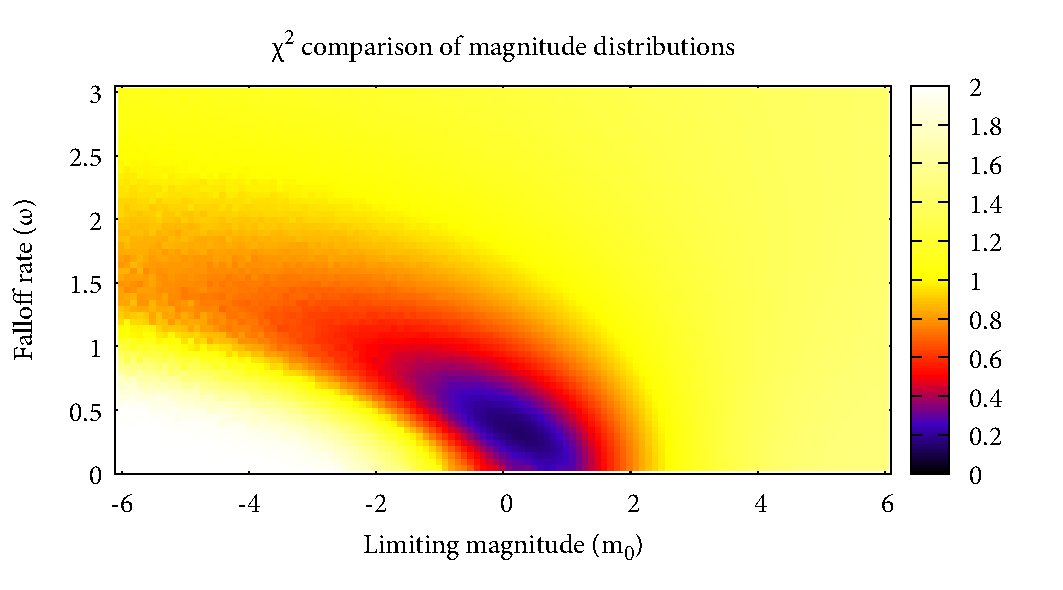
\includegraphics[width = 0.875\paperwidth]{chiSquare-magnitude-1d8.pdf}
            }
            \frejm{Heatmap -- zooming in}{
                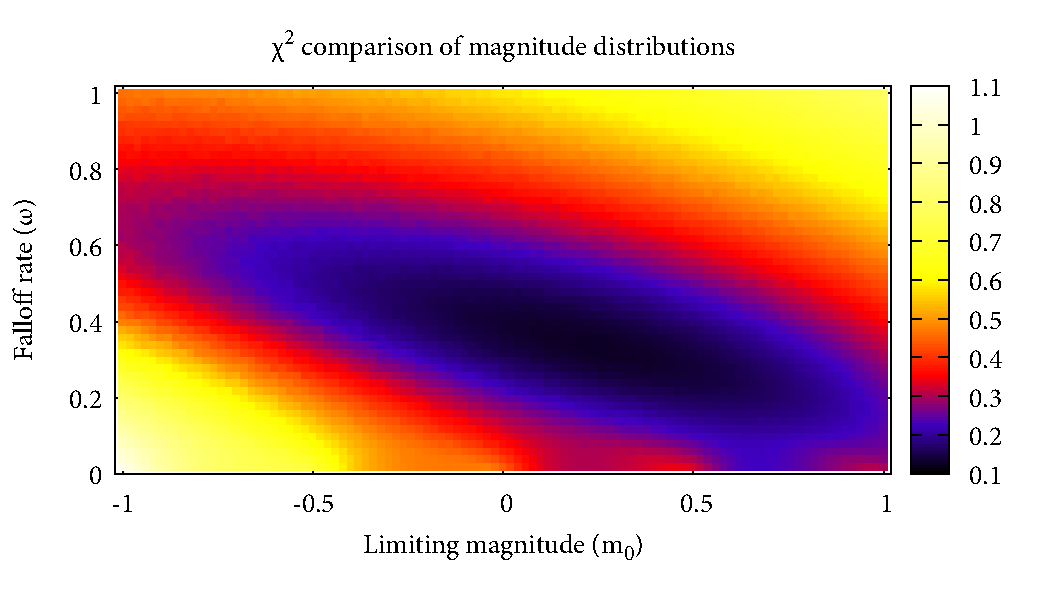
\includegraphics[width = 0.875\paperwidth]{chiSquare-magnitude-1d8z.pdf}
            }
			\fspicture{best.pdf}[][white]
			
			\frejm{Mass index $s$}{
				There are too many bright meteors...
				\pause
				\begin{itemize}                
					\item a natural reaction is to try other values of $s$
					\begin{itemize}
						\item a full range \numrange{1.6}{2.8} was tried
					\end{itemize}
					\item best fit for $s = \text{2.15}$
                    \pause
                    \item \emph{no value below 2 consistent with observations}
				\end{itemize}
			}        
			\fspicture{bestofbest.pdf}[][white]
			
			\frejm{DPF for altitude and angular speed}{
				$$
					A(\theta; \alpha) = \left(\sin \theta\right)^\alpha
				$$
				\begin{itemize}                
					\item only a simple 1D fit for $\alpha$
					\item a well defined minimum at $\alpha = \text{0.4}$
				\end{itemize}
                \vspace*{8mm}
                \pause
                \begin{itemize}
                    \item no discernible optimum for angular speed DPF
                \end{itemize}
                $$
                    S(\omega) \equiv 1
                $$
			}
    
    \section{Results}    
		\subsection{Results}    
			\frejm{Total flux}{
				Finally, we may calculate the total flux
                \pause
				\begin{itemize}
					\item simulation is run again with AMOS's \emph{optimal DPF parameters}
                        $$A(\theta) = \left(\sin \theta\right)^{0.4} \qquad D(m) = \frac{0.93}{1 + e^{\frac{m + 0.17}{0.362}}} \qquad S(\omega) \equiv 1$$
					\item the number of meteors is \emph{scaled} to match observations
                    \item this should correspond to the real population
				\end{itemize}
				\pause
				\begin{itemize}
					\item \num{135000} particles per \SI{1000000}{\kilo\metre\squared\hour}
					\item \SI{0.338}{\kilo\gram} per \SI{1000000}{\kilo\metre\squared\hour} $\approx$ \SI{43}{\kilo\gram\per\hour} over entire Earth
				\end{itemize}
			}
			
			\frejm{Comparison}{
				\begin{itemize}
					\item results consistent with recent estimates
					\begin{itemize}
						\item \emph{Blaauw et al., 2016}: \num{98000} particles per \SI{1000000}{\kilo\metre\squared\hour}
						\item \emph{Molau, 2017}: \num{47000} particles per \SI{1000000}{\kilo\metre\squared\hour} (up to 6.5$^\text{m}$)
					\end{itemize}
					\item but a high fraction of small particles ($s = \text{2.15}$)
				\end{itemize}
				\pause
                \begin{itemize}
                    \item but we still need
                    \begin{itemize}
                        \item multiparametric evaluation
                        \item a larger observational dataset
                        \item detailed camera calibration
                    \end{itemize}
                \end{itemize}
			}
							
    \section{Conclusion}
		\subsection{Conclusion}
			\frejm{Summary}{
				\begin{itemize}
					\item it is a \emph{surprisingly good} method
					\begin{itemize}
                        \item versatile, universal tool
						\item applicable to \emph{almost any} meteor observing system
					\end{itemize}
				\end{itemize}
				\pause
				\begin{itemize}
					\item we were able to estimate the \emph{flux}
					\begin{itemize}
						\item mass index seems higher than known values
                        \item but consistent with our expectations
					\end{itemize}
				\end{itemize}
                \pause
				\begin{itemize}
                    \item the tools will be \emph{shared} and free to use
                    \item any comments or suggestions are welcome
				\end{itemize}
			}
			
			\frejm{References}{
				\begin{itemize}
					\item \textbf{Öpik, E. J.}:
						Physics of meteor flight in the atmosphere. Interscience Publishers, 1958.  
					\item \textbf{Jenniskens, P.}:
						Meteor Showers and Their Parent Comets. Cambridge University Press, Cambridge, 2006.
					\item \textbf{Blaauw, R. C. et al.}:
						Optical meteor fluxes and application to the 2015 Perseids. MNRAS vol. 463, 2016, pp441--448.
					\item \textbf{Hill, K. A. -- Rogers, L. A. -- Hawkes, R. L.}:
						High geocentric velocity meteor ablation. Astronomy \& Astrophysics 444, 615--624 (2005) 
                    \item \textbf{Jones, W. -- Halliday, I.}:
                        Effects of Excitation and Ionization in Meteor Trains. MNRAS vol. 321, 2001, pp417--423.
				\end{itemize}
			}
				
\end{document}
